% Copyright 2020 by Robert Hildebrand
% Adapted from https://tex.stackexchange.com/questions/394923/how-one-can-draw-a-convex-function
% from response by jpayansomet, Creative Commons CC-BY-SA
%This work is licensed under a
%Creative Commons Attribution-ShareAlike 4.0 International License (CC BY-SA 4.0)
%See http://creativecommons.org/licenses/by-sa/4.0/



\documentclass[tikz,border={15mm 15mm 15mm 15mm},]{standalone}
\usepackage{pgfplots} 
\pgfplotsset{compat=newest}
\pgfplotsset{plot coordinates/math parser=false}
\pgfplotsset{
    every non boxed x axis/.style={
        xtick align=center,
        enlarge x limits=true,
        x axis line style={line width=0.8pt, -latex}
},
    every boxed x axis/.style={}, enlargelimits=false
}
\pgfplotsset{
    every non boxed y axis/.style={
        ytick align=center,
        enlarge y limits=true,
        y axis line style={line width=0.8pt, -latex}
},
    every boxed y axis/.style={}, enlargelimits=false
}
\usetikzlibrary{
   arrows.meta,
  intersections,
}
\begin{document}
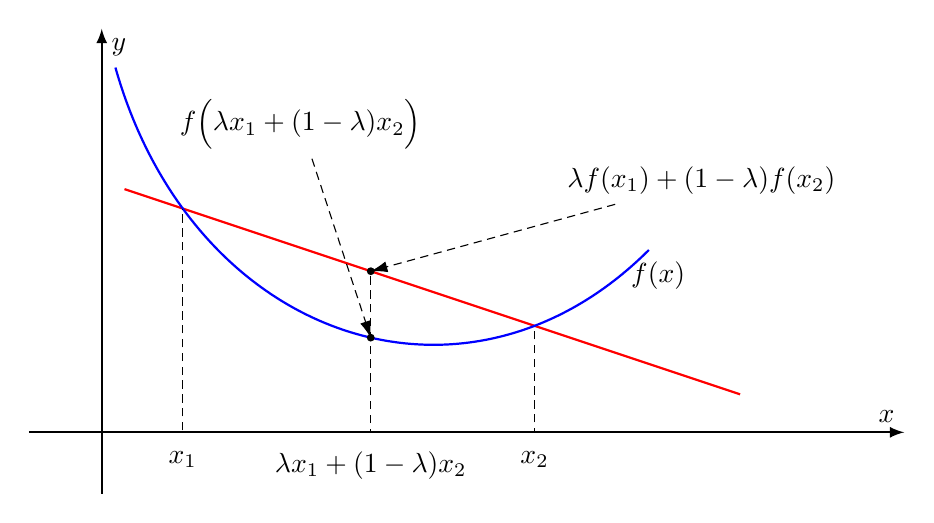
\begin{tikzpicture}
\begin{axis}[width=5in,axis equal image,
    axis lines=middle,
    xmin=0,xmax=8,
    xlabel=$x$,ylabel=$y$,
    ymin=-0.25,ymax=4,
    xtick={\empty},ytick={\empty}, axis on top
]

% 
\addplot[thick,domain=0.25:7,red,name path = A]  {-x/3 + 2.75} coordinate[pos=0.4] (m) ;
\draw[thick,blue, name path =B] (0.15,4) .. controls (1,1) and (4,0) .. (6,2) node[pos=0.95, color=black, right]  {$f(x)$} coordinate[pos=0.075] (a1)  coordinate[pos=0.95] (a2);
\path [name intersections={of=A and B, by={a,b}}];

% 
%\draw[densely dashed] (0,0) -| node[pos=0.5, color=black, label=below:$a$] {}(a1);
\draw[densely dashed] (0,0) -| node[pos=0.5, color=black, label=below:$x_{1}$] {}(a);
\draw[densely dashed, name path=D] (3,0) -|node[pos=0.5, color=black, label=below:$\lambda x_{1}+ (1-\lambda)x_{2}$] {} node[pos=1, fill,circle,inner sep=1pt] {}(m);
\draw[densely dashed] (0,0) -|node[pos=0.5, color=black, label=below:$x_{2}$] {}(b);
%\draw[densely dashed] (0,0) -|node[pos=0.5, color=black, label=below:$b$] {}(a2);

% 
\path [name intersections={of=B and D, by={c}}] node[fill,circle,inner sep=1pt] at (c) {}; 

% 
\node[anchor=south west, text=black] (d) at (0.75,3) {$f\Big(\lambda x_{1}+(1-\lambda)x_{2}\Big)$};
\node[anchor=south west, text=black] (e) at (5,2.5) {$\lambda f(x_{1})+(1-\lambda)f(x_{2})$};
\draw[-{Latex[width=4pt,length=6pt]}, densely dashed] (d) -- (c);
\draw[-{Latex[width=4pt,length=6pt]}, densely dashed] (e) -- (m);
\end{axis}
\end{tikzpicture}

\end{document}
